%************************************************
\chapter{Patterns of sitewise selection in mammalian protein-coding genes}\label{ch:mammals1}
%************************************************

\section{Introduction}

\subsection{The Mammalian Genome Project}

A major goal of mammalian comparative genomics has been to quantify,
identify and understand the fraction of the human genome that is under
evolutionary constraint. The first non-human mammalian genomes showed
at least 5\% of the human genome to be under purifying selection
\citep{Mouse2002Initial,Rat2004Genome,LindbladToh2005Genome}, but the
small number of genomes available limited the extent to which regions
of evolutionary constraint could be identified. The \mgp, a
coordinated set of genome sequencing projects initiated in 2005 and
organised by the Broad Institute of MIT and Harvard, was designed with
the primary purpose of increasing the accuracy and confidence with
which regions of the human genome that have evolved under evolutionary
constraint in mammals could be identified \citep{TODO}. In line with
this goal, 20 mammalian species were chosen for sequencing in order to
maximise the amount of evolutionary divergence available for
comparative analysis when combined with the 9 already available
sequenced genomes \citep{Margulies2005Initial}. Importantly, to save
on sequencing costs most of the 20 additional species were only
sequenced to a target twofold coverage, meaning each genomic base pair
would be covered on average by two sequence reads and roughly 85\% of
genomic sequence would be covered by at least one read.

As the \mgp proceeded from its sequencing to analysis phase in late
2008, it became clear that the additional branch length afforded by
the 29-species phylogeny would enable a number of improved
evolutionary analyses beyond the identification of constrained
noncoding regions. Among others, these included the evolutionary
characterisation of gene promoters, identification of exapted
noncoding elements, detection of evolutionary acceleration and
deceleration in noncoding regions, and detection of purifying and
positive selection in protein-coding genes. Given its prior
involvement in analysing the ENCODE comparative sequencing data
\citep{TODO} and Massingham's work on a method and software program
for sitewise evolutionary analysis \citep{TODO}, the Goldman group
became involved in the protein-coding evolutionary analysis for the
\mgp. This chapter describes my work on the project, which began in
late 2008; the major results from the analysis are to be published in
\citep{TODO}, and all of the work described below was performed by me
in consultation with members of the Goldman group (Nick Goldman and
Tim Massingham), EnsEMBL team (Albert Vilella, Javier Herrero, Ewan
Birney) and organisers and members of the \mgp (Manolis Kellis,
Kerstin Lindblad-Toh, Mike Lin, Katie Pollard).

\subsection{The Sitewise Likelihood Ratio test}

As described in Chapter \ref{ch_bg}, differential survival of \nsyn
and \syn mutations based on the degeneracy of the genetic code can be
used as a source of information on the continued importance of
mutations at a given protein-coding site over evolutionary time: a
lower rate of \nsyn substitution compared to \syn substitution is
indicative of purifying selection, or natural selection in favor of
maintaining protein structure and function; equal rates of \nsyn and
\syn substitutions is indicative of neutral selection, or no
differential survival of protein-altering mutations; a greater rate of
\nsyn than \syn substitution is indicative of positive selection, or
natural selection in favor of protein-altering mutations.

Early evolutionary analyses of protein sequences showed large
variation in the rates of amino acid change both within and between
proteins \citep{TODO}. This variety results from the myriad structures
and functions embodied by different proteins and protein domains
\citep{TODO}. Continued work suggested that the overall evolutionary
rate \cite{TODO,Koonin?} and the pattern of localised selective
pressures \cite{TODO} of a gene can reveal important insight into its
role in the organism. Thus, the study of rates of \nsyn and \syn
substitution in proteins became established as an effective method for
using evolutionary information to investigate the functional
characteristics of genes.

Maximum likelihood methods, introduced in Chapter \ref{TODO}, are
commonly applied to biological sequence analysis due to their
desirable statistical features...

The Sitewise Likelihood Ratio (SLR) test is based on the mechanistic
Goldman-Yang codon model of evolution, with an additional parameter
for each site in the alignment representing the sitewise $\omega$
value. The inclusion of an additional parameter per alignment site
makes the model extremely complex and difficult to optimise, but the
dimensionality of the likelihood optimisation is reduced by making the
assumption that the $\omega$ at each site does not contribute
significantly to the overall likelihood, thus allowing for separate
optimisation of the global parameters (including XYZ) across the whole
alignment and the $\omega$ parameter at each site. In this way, SLR
performs an approximate likelihood ratio test (LRT) for non-neutral
evolution at each site...

\subsection{Data quality concerns: alignment and sequencing error}

The possibility that errors in the source alignments might cause false
positives in the detection of sitewise positive selection was a major
concern for this analysis. Although the SLR test and other \sw \ml
methods have been shown to be conservative for detecting positive
selection even when the amount of data is low or the null model is
violated \citep{Anisimova2002Properties,Massingham2005Detecting,TODO},
most evolutionary analyses are based on the assumption that all sites
within an alignment column are truly homologous. This assumption can
be violated in a number of ways, some of which are described below.

Alignment error results from the difficulty of reconstructing the
evolutionary history of sequences evolving with indels and can cause
nonhomologous codons to be placed in the same alignment column. In
Chapters \ref{ch_indel1} and \ref{ch_indel2} I explored the tendency
of multiple aligners to produce such errors, showing that \prankc
alignments would be expected to introduce few falsely identified
positively-selected sites resulting from alignment errors at
mammalian-like divergence levels.

Errors resulting from incorrect genomic sequence was an additional
concern. Twenty of the genomes under study were sequenced at low
coverage and were not assembled into chromosomes or finished to
completion, making the likelihood of miscalled bases, spurious
insertions or deletions, or shuffled regions due to misassembly
relatively high \citep{TODO}. The potential effect of each of the
aforementioned types of sequence errors on the detection of positive
or purifying selection depends on the nature of the inference method,
the type of sequencing error, and the branch length of the terminal
lineage leading to the species containing the error.

As most codon-based inference methods assume independence between
amino acid sites, I first consider the effect---in isolation---of a
single spuriously-assigned homologous codon on the \ml estimation of
$\omega$. Two cases can be considered: a single sequence error causing
one spurious substitution within a codon, and one or multiple sequence
or assembly errors causing multiple spurious substitutions within a
codon. In the case of a single spurious substitution, if we assume no
large difference between the natural mutational process and the
process that caused the erroneous mutation, then the effect would be
to shift the estimated $\omega$ in the branch containing the error
towards 1. The sequence error would be incorporated into the \ml
optimisation as an additional neutral substitution, inflating the
estimated substitution rate but not affecting the relative \nsyn and
\syn rates. This effect may be biased towards higher or lower $\omega$
values if a significant difference exists between the neutral
biological mutational process and the pseudo-mutational process
causing the erroneous substitution. On the other hand, a codon with
multiple erroneous bases may cause greater elevation of the inferred
substitution rate and $\omega$, due to the necessity of \ml methods to
infer a multi-step path of single substitutions between the two codons
on either side of a given evolutionary branch. The path estimated
between two completely nonhomologous codons depends on the estimated
codon frequencies, the genetic code, and the pseudo-mutational
process; while a detailed investigation of the expected effect on
inferred $\omega$ values is beyond the scope of my analysis, it is not
unreasonable to expect a greater number of false positive \pss{}s
resulting from codons with multiple erroneous bases than from codons
with single errors.

{\color{red} TODO: quick randomisation experiment looking at elevated
  $\omega$ from multi-substitution codons?}

Given the potentially greater impact of codons with multiple errors,
the propensity of each of the common sequencing error types identified
above (miscalled bases, spurious indels, and
shuffled/repeated/collapsed regions due to mis-assembly) to cause
single or multiple errors within codons could strongly affect its
effect on the detection of positive selection. On its own, a miscalled
base would obviously result in a single spurious
substitution. However, low-quality bases tend not to be uniformly
distributed among or within sequence reads, which makes for a larger
probability of multiple errors within a codon resulting from miscalled
bases. Spurious indels within coding regions may be even more likely
than miscalled bases to cause multiple errors within a codon due to
the potential alignment and frameshift effects (but see the discussion
of Ensembl's frameshift filters for low-coverage genomes in Section
\ref{TODO}). Assembly errors, which result in larger-scale structural
errors including missing, repeated, shuffled or inverted sequence
regions, are most prone to produce codons with multiple erroneous
errors due to the large amount of contiguous sequence data being
misplaced.

I also note the impact of the inference method and terminal branch
length on false positives resulting from sequence errors, which can be
understood in terms of the information most directly affecting the
inference of a positively selected site or a positively selected gene
for a given detection method. Both the branch-site test and the
sitewise tests (including \slr and \pamlEight) are sensitive to
substitutions at a subset of alignment sites, but the branch-site test
is specifically sensitive to substitutions along the foreground
branches of interest while the sitewise tests detect positive
selection only throughout the entire tree. In the latter case, the
effect of spurious \syn and \nsyn substitutions from sequence data
depends on the ratio of the species' terminal branch length to the
branch length of the entire tree: a longer terminal branch gives
greater weight to the erroneous sequence data, making false positives
more likely to result. In the former case of the branch-site test, the
potential effect depends on the location and length of the foreground
branches. If the terminal branch leading to the spurious sequence is
within the foreground and the total foreground branch length is small,
then false positives could easily result; if, however, the terminal
branch is outside of the foreground then it should have little to no
effect on the \fpr of the branch-site test. Interestingly, this
suggests that branch-site tests where the foreground only consists of
internal branches may be less prone to false positives from sequencing
error than tests that include terminal lineages in the foreground
model.

To summarise, the expected effect of alignment errors on the sitewise
detection of positive selection should be minimal when using a good
aligner and analysing data within vertebrate divergence levels, but
the number of false positives resulting from sequence errors depends
on a number of factors including the frequency, spatial clustering,
and phylogenetic branch length associated with sequencing-based errors
when applied to detecting sitewise positive selection. In some cases
even a large amount of sequencing error should not produce a strongly
elevated \fpr (e.g., when the total branch length is large, when
analysing all mammals or vertebrates) but in other cases it could
potentially bias results (e.g., when the branch length is small and/or
many low-quality genomes are included, as in the major mammalian
sub-clades).

Simulation studies similar to those I performed in Chapters
\ref{ch_indel1} and \ref{ch_indel2} could improve our understanding of
the relative potential of different types of sequencing errors to
introduce false positives in downstream analyses, but the absolute
frequency and pattern of such errors would still difficult to predict
without a reliable model for their generation. This is especially true
for larger-scale errors from misassembly or misannotation, which are
less easily modeled than base calling errors and could have
potentially larger negative effects. For estimates of false positives
resulting from these types of sequence errors, an empirical approach
seems more appropriate.

Two empirical studies in mammals have provided convincing evidence
that sequence, alignment and annotation errors can drastically
increase the number of false positive \psg{}s in the branch-site test
for positive selection.

Schneider et al. \citeyearpar{Schneider2009Estimates} performed a
genome-wide scan for positive selection in the terminal branches of 7
mammalian genomes using the branch-site test and analysed the fraction
of \psg{}s within subsets of high- or low-quality genes according to
three sequence and alignment quality metrics. They found that the
fraction of \psg{}s was significnatly higher for genes exhibiting
lower quality sequence, annotation and alignment metric, with genes in
the highest-quality and lowest-quality categories showing a 7.2-fold
difference in the inferred fraction of \psg{}s
\citep{Schneider2009Estimates}. This observation provided evidence of
a correlation between the chosen quality metrics and the tendency of
an alignment to exhibit positive selection. It did not necessarily
imply causation, however, as the same result might have been
observed---even in the absence of sequence error---if some biological
properties of the true \psg{}s caused them to yield lower quality
metrics than non-\psg{}s. Looking at the three metrics used in their
study (sequencing coverage, gene annotation status, and alignment
quality according to the heads-or-tails method), it is plausible that
properties associated with elevated $\omega$ ratios and positive
selection, such as recent gene duplication \citep{TODO}, high GC
content \citep{TODO} or functional shifts \citep{TODO} might have had
an error-independent effect resulting in a higher proportion of
\psg{}s in low-scoring categories.

Mallick et al. \citeyearpar{Mallick2009Difficulty} took a different
approach to the same problem by performing a careful resequencing and
reassembly of the chimpanzee genome (the initial assembly of which had
lower coverage and lower quality than the human genome) and
re-analysing the evidence for positive selection along the chimpanzee
linegae in 59 genes which had previously been identified as chimpanzee
\psg{}s. The authors, who were motivated by a concern that previous
reports of a larger proportion of \psg{}s in chimpanzee than in human
\citep{TODO} were the result of its lower-quality genome rather than a
biologically significant difference in levels of adaptation, found
that the vast majority of \psg{}s identified in two previous studies
showed no evidence for positive selection when using their reassembled
and higher-coverage version of the chimpanzee genome
\citep{Mallick2009Difficulty}. This suggested that the original 4x
coverage chimpanzee assembly contained a number of sequencing errors
leading to false inferences of positive selection. A detailed analysis
of 302 codons with multiple spurious \nsyn substitutions in the
original assembly showed roughly comparable effects of sequence error
(explaining 23\% of codons), assembly error (14\% of codons) and local
alignment error (30\% of codons).

Taken together, the results of Schneider et
al. \citeyearpar{Schneider2009Estimates} and Mallick et
al. \citeyearpar{Mallick2009Difficulty} provide strong evidence in
support of the hypothesis that errors in sequencing, assembly,
annotation and alignment can result in strongly elevated inferred
$\omega$ values when using sensitive tests for detecting positive
selection. The detailed identification and quantification of error
sources performed by Mallick et
al. \citeyearpar{Mallick2009Difficulty} is especially useful for
designing filters to apply to an analysis based largely on
low-coverage genomes; their observation that clusters of
chimpanzee-specific mutations were responsible for many false
positives motivated the window-based filter I applied here and in
Chapters \ref{ch_gorilla1} and \ref{ch_gorilla2}.

{\color{red} TODO: Figure summarising the types of error and potential effects on the inference?}

\subsection{Low-coverage genomes in the Ensembl database}

The prevalence of missing sequence data and fragmented contigs in
low-coverage genomes presents a unique set of problems for the
generation of transcript annotations. In recognition of these
differences, the procedure used by the Ensembl database to annotate
genomes assembled from low-coverage data is distinct from the usual
gene-building pipeline \citep{TODO, Ensembl 2006}. Briefly, a
whole-genome alignment is produced between the human genome and each
low-coverage target, and gene models are projected from human to the
target genome. Small frame-disrupting insertions or deletions within
orthologous exons are corrected, and missing exons are padded with Ns
in order to obtain the correct transcript length.

The inclusion of these error-correcting features allows intact, if not
complete, coding transcripts to be generated for low-coverage
genomes. The Compara gene family pipeline uses the set of transcripts
from each species as its input \citep{TODO, Ensembl Compara}, so the
quality of the gene models from each species has a direct impact on
the overall quality and accuracy of gene trees. Although the reliance
on genome-wide alignments to, and gene annotations from, a reference
genome could be criticised for potentially causing a bias towards the
genomic properties of the reference, this approach is a reasonable
workaround in the absence of higher-coverage sequence data or a
painstakingly curated assembly. Furthermore, the gene model error-correcting
features of the Ensembl pipeline are especially beneficial, making
more complicated methods for correcting errors from low-coverage
genomes such as those described by \citep{TODO, PLoS One hubisz and
  siepel} seem largely unnecessary.

\section{Source data and methods}

All genomic data and gene trees used for this analysis were sourced
from version 63 of the Ensembl Compara database \citep{TODO, Ensembl
  2010 and EnsemblCompara GeneTrees}. Although a complete description
of the design, implementation, and validation of the pipeline behind
the Ensembl database is beyond the scope of this thesis, I will
briefly outline the major aspects of the approach and some details
which are relevant to my sitewise analysis and the ensuing discussion.

The Compara pipeline begins with a set of protein-coding transcripts
collected from each individual species' annotation database. This step
is not exactly straightforward, as the prevalence of alternative
splicing in Eutherian mammals makes it common for a single gene to
harbor many different transcript structures. In terms of biology and
evolution, alternative splicing is a very interesting
phenomenon. Tightly linked to the evolutionary innovation of
regulatory control and tissue-specific gene expression, the existence
of multiple transcripts per gene is one of the likely substrates of
biological and developmental complexity within eutherian mammals as
compared to single-celled eukaryotes, which show less developmental
complexity but largely similar numbers of genes \citep{TODO}. However,
in terms of organizing biological data, pervasive alternative
splicing---with up to dozens of transcripts per gene, showing
tissue-specific and species-specific expression patterns, different
levels of overall transcription, and sometimes comprising mutually
exclusive exons---is somewhat burdensome. 

\subsection{Identifying orthologous subtrees within large mammalian gene families}

The first step in 

\subsection{Filtering out low-quality genome sequence}




\subsection{Filtering out clusters of \nsyn substitutions}


\section{Analysis of the genome-wide set of orthologous mammalian trees}

\begin{figure}[t]
\begin{center}
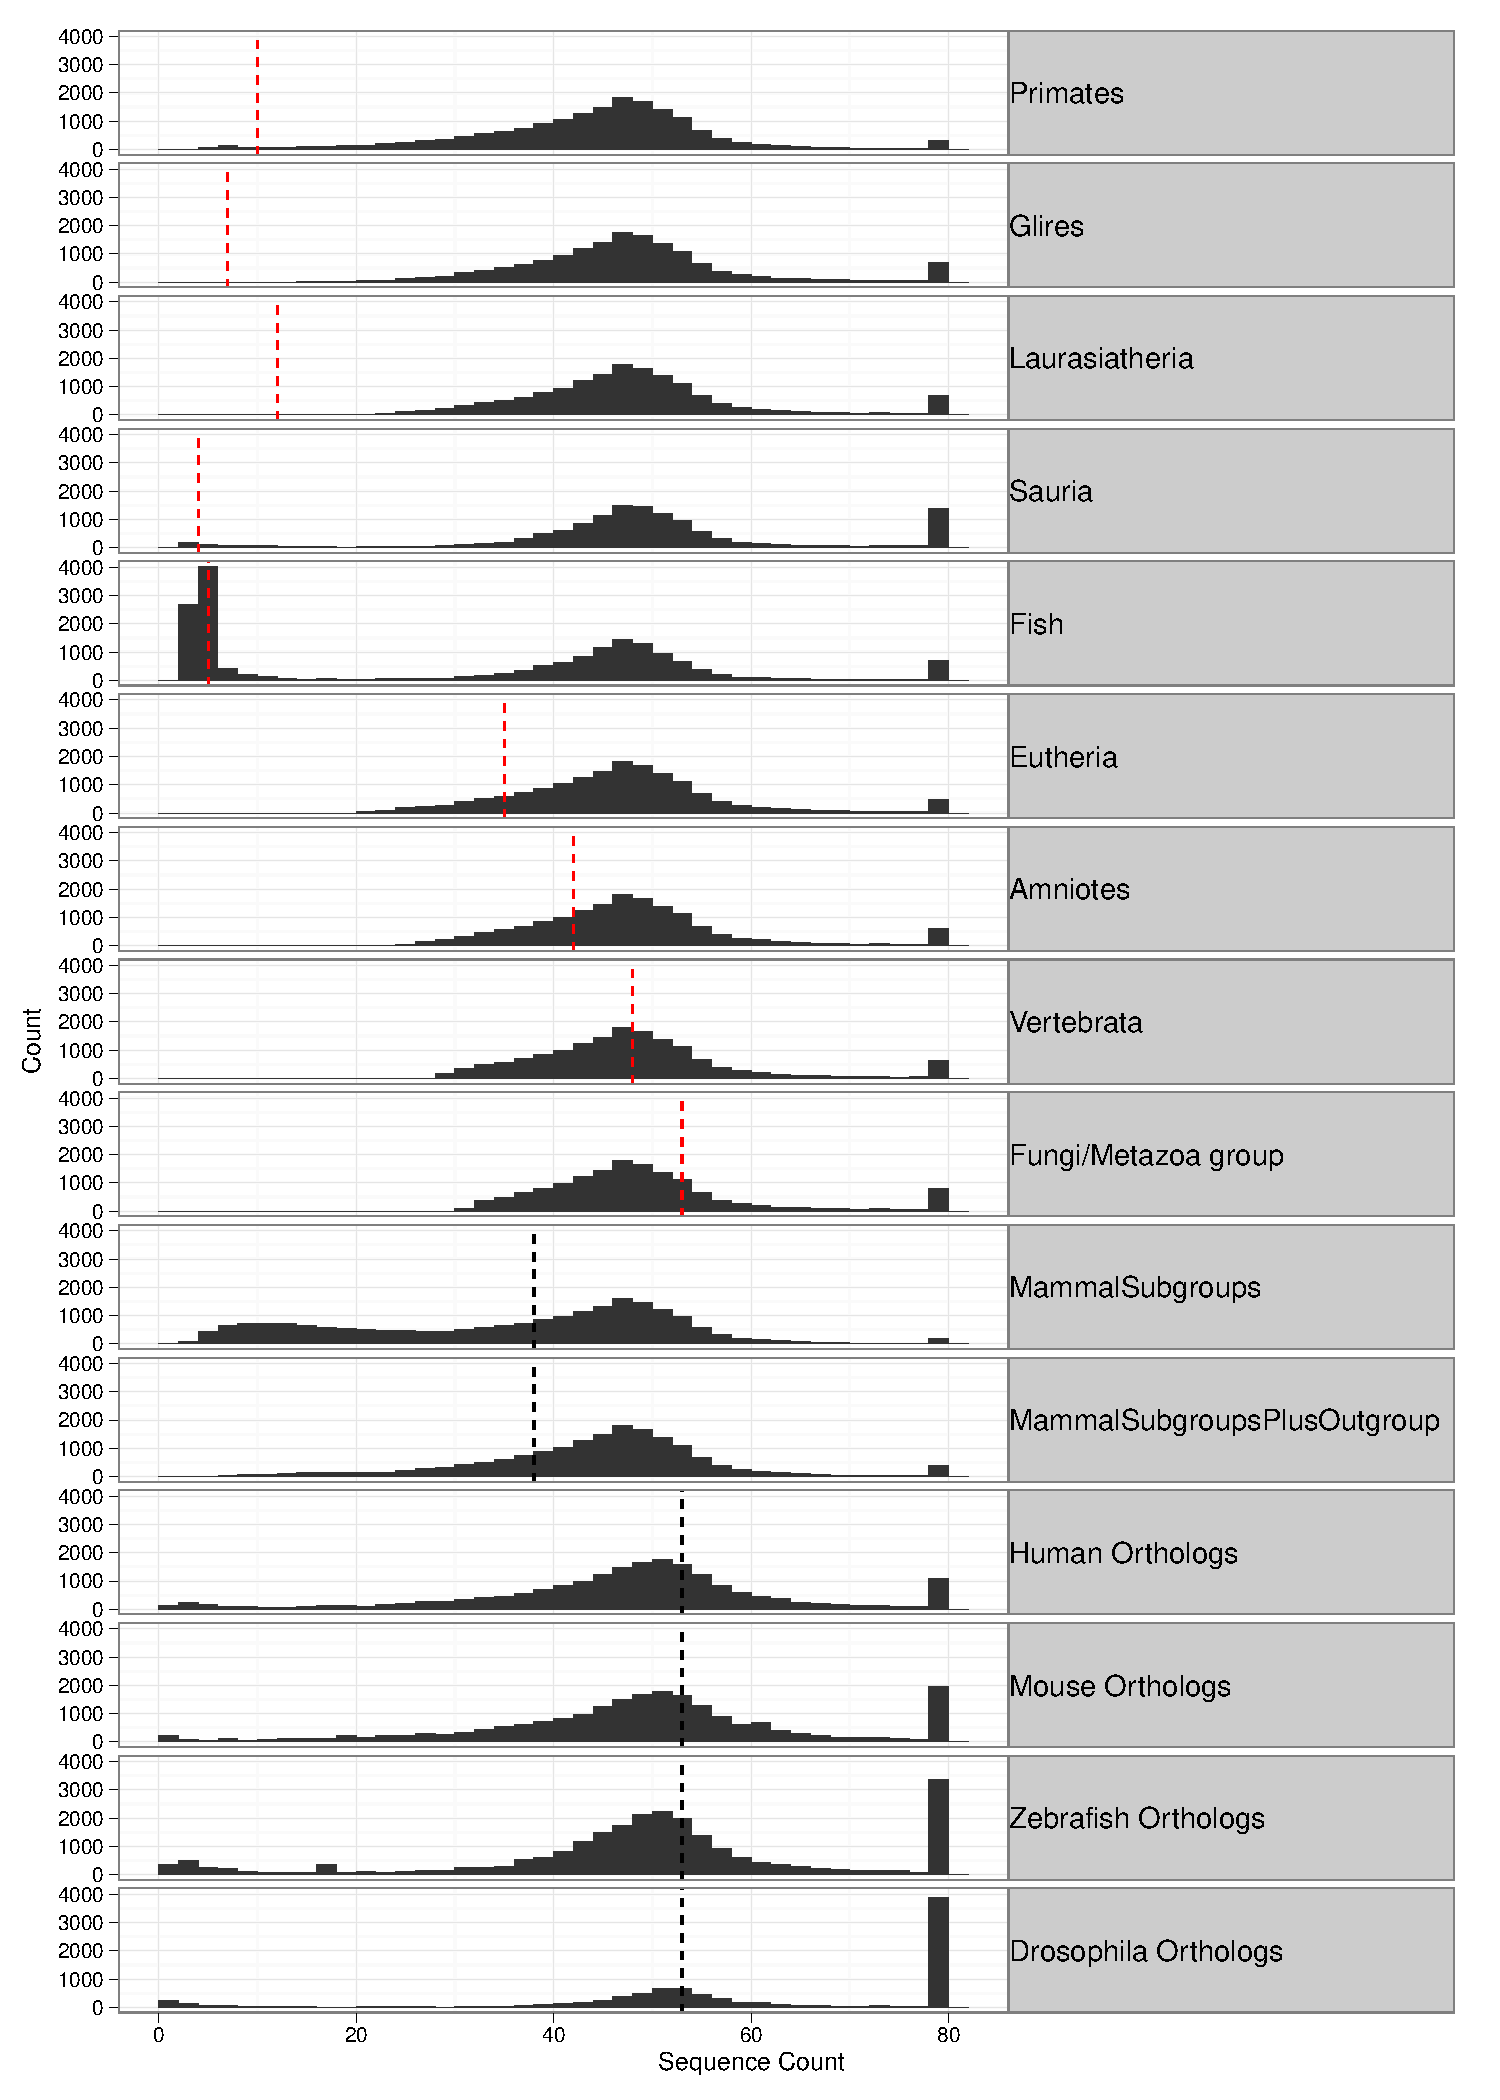
\includegraphics[scale=0.6]{Figs/Mammals1_Fig1.pdf}
\end{center}
\caption{Histogram of gene tree sizes for the different node delineation methods. }
\label{mammals1_fig1}
\end{figure}

\begin{figure}[t]
\begin{center}
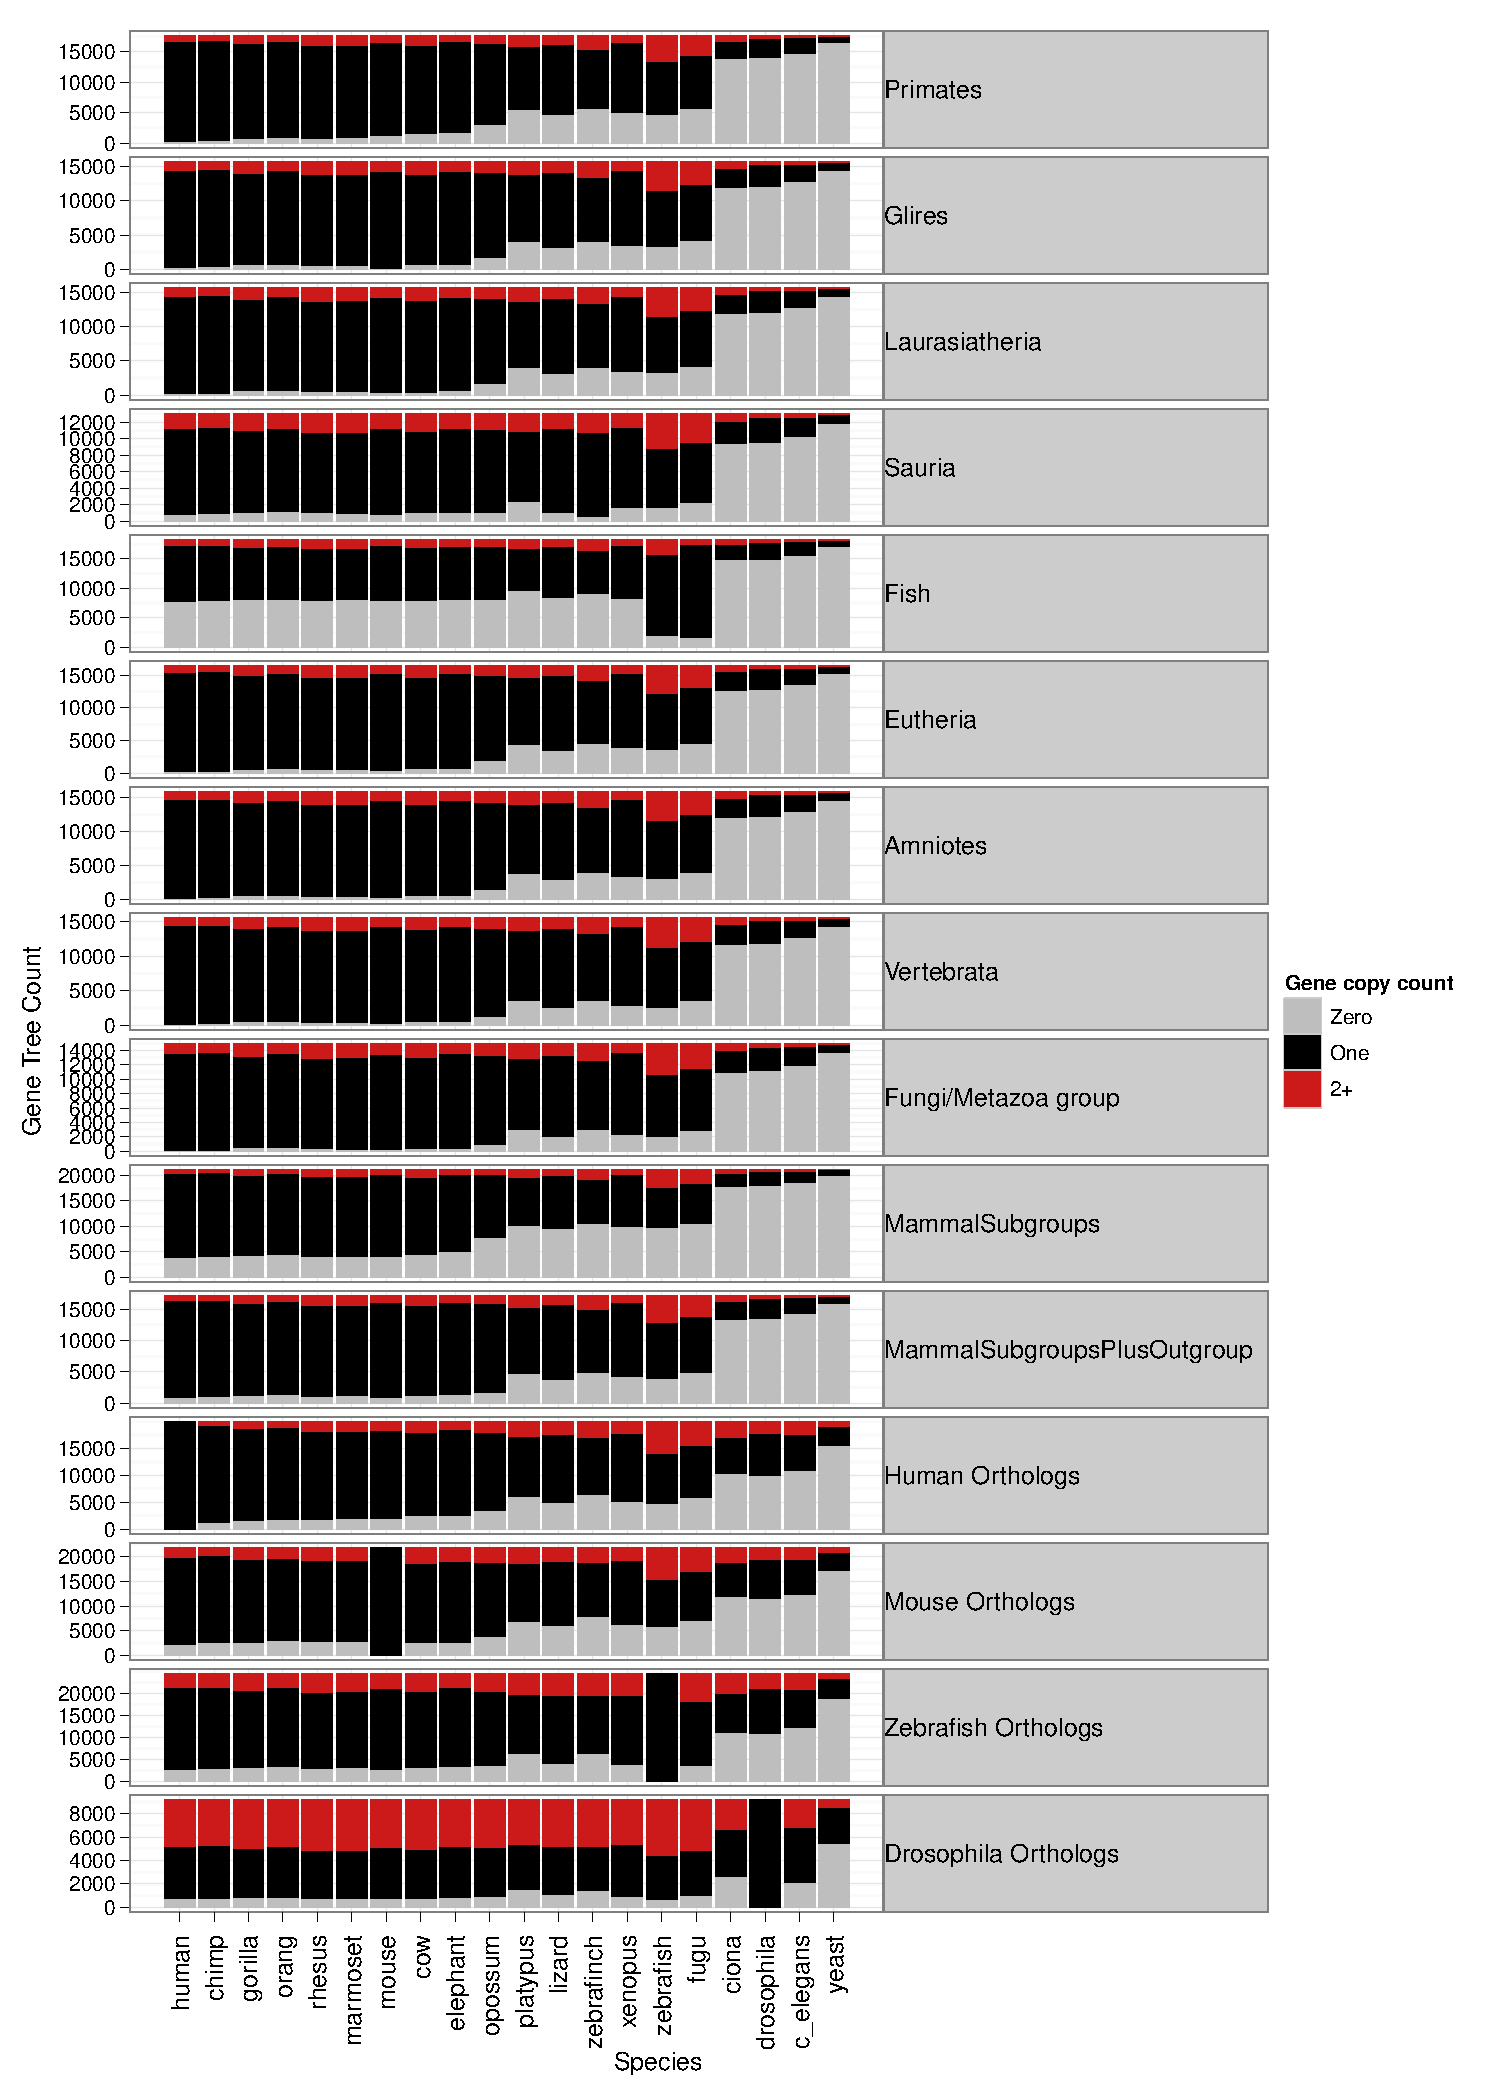
\includegraphics[scale=0.6]{Figs/Mammals1_Fig2.pdf}
\end{center}
\caption{Barplot of gene copy counts for mammalian species using different node delineation methods.}
\label{mammals1_fig1}
\end{figure}

\begin{figure}[h]
\begin{center}
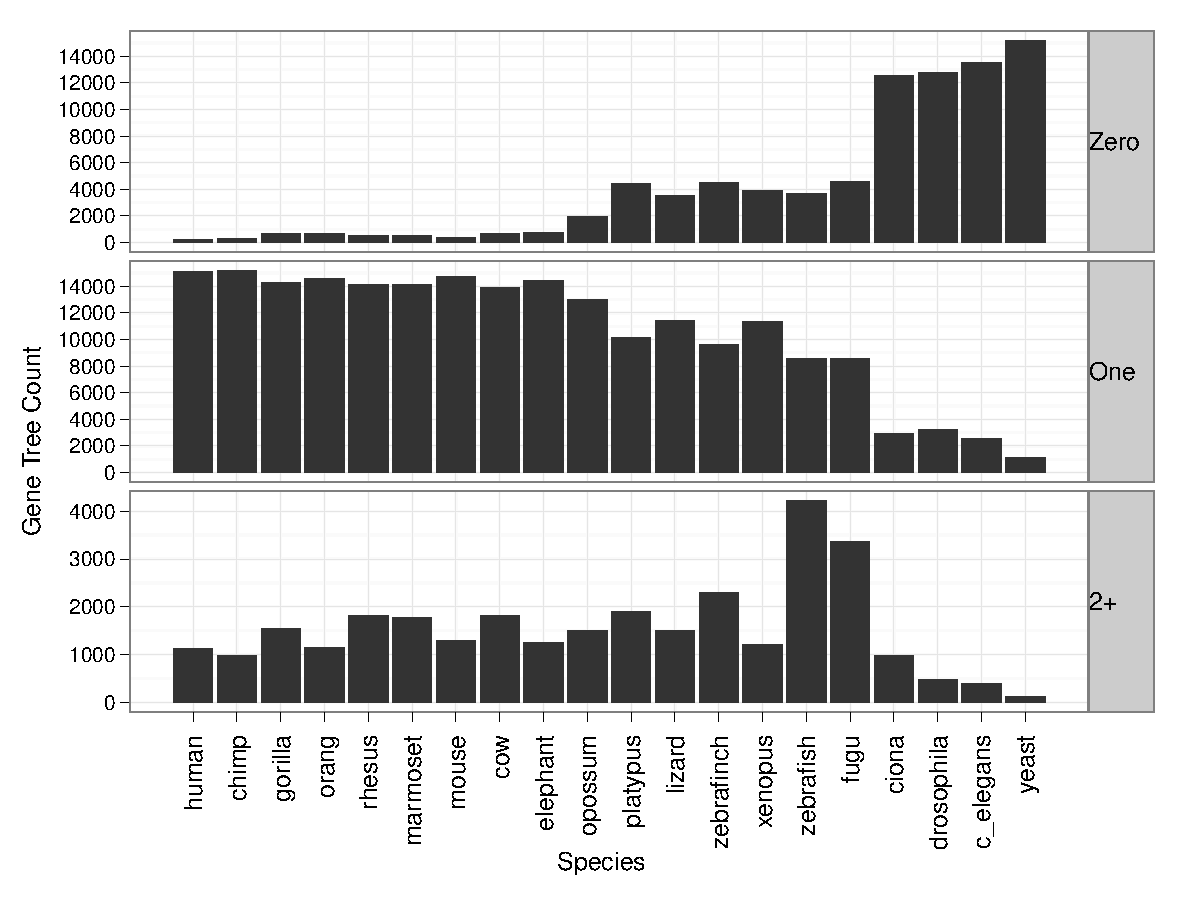
\includegraphics[scale=0.6]{Figs/Mammals1_Fig3.pdf}
\end{center}
\caption{Gene copy counts for mammalian species using the Eutherian node delineation method.}
\label{mammals1_fig1}
\end{figure}

\section{Analysis of the global distribution of mammalian selective pressures}



\section{Analysis of sitewise estimates from three mammalian sub-clades}



\section{Evaluation of the effect of GC content, recombination rate, and codon usage on sitewise dnds estimates and the detection of positive selection}



\subsection{Mammalian sitewise selective pressures are not subject to strong effects of biased gene conversion}



\subsection{Mammalian sitewise selective pressures suggest increased efficacy of natural selection in regions of high recombination}



\section{Conclusions and future work}
